\chapter{Design}\label{chp:reqdes}
The principal aim of the project is to create a system that allows the generation of network data to train an anomaly-based intrusion detection system. The system, therefore, comprises three primary parts: data generation, data processing and data modelling. 

\section{Overall System Design}
\begin{figure}[H]
\centering
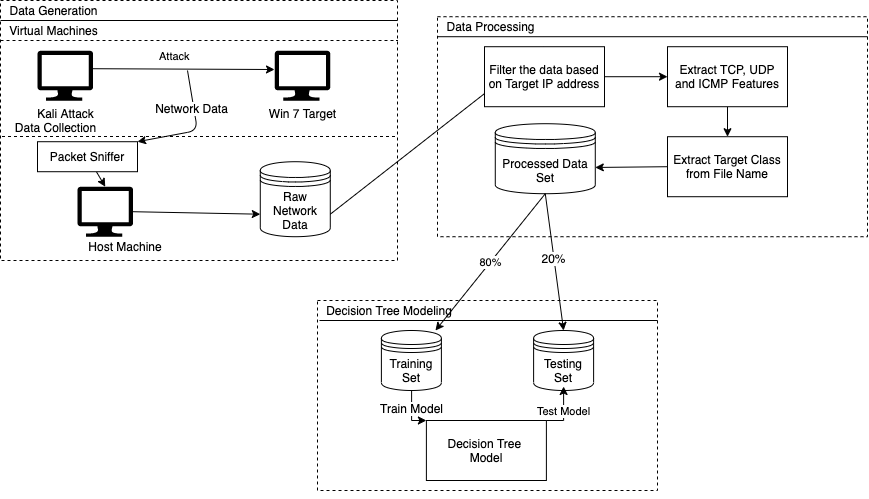
\includegraphics[scale = 0.45]{Images/Mainsystem.png}
\caption{Overall System Diagram}
\label{fig:osd}
\end{figure}

The systems diagram in Figure \ref{fig:osd} shows the 3 separate sections of the system and how they interconnect. Each module is built to the specifications defined in chapter \ref{chp:req}. The user may replace these \ depending on their specifications. 

\begin{itemize}
\item The data generation phase should allow the spinning of virtual machines, these virtual machines should then simulate an attack scenario. The network data from the attacks should then be collected by the host PC and stored as raw network data, the file name corresponding to the attack which has been made.
\item The data collection phase should process the data first by filtering IP addresses to only leave the packets the virtual machines have sent or received. Next, it must extract the TCP, UDP, and ICMP packets and their features. These packets should be collated every second to form the processed data set. The data will be labelled based on the file name. 
\item The decision tree modelling phase should split the dataset into training and testing sets and train a decision tree on the data. The model will be tested here and extracted for future use.
\end{itemize}

\section{Data Generation}\label{sec:datagen}
This part of the project is focused on the generation of raw network data. This will first be achieved by creating a virtualised network where the attacks will take place. The project uses a virtualised network, rather than a physical network made of hardware, because most attacks are designed to be harmful to the hardware that it attacks. Using a virtualised network allows the attacks to take place away from any hardware and leave no lasting effect. The plan for this module can be seen in Figure \ref{fig:dgd}.
\begin{figure}[H]
 \centering
 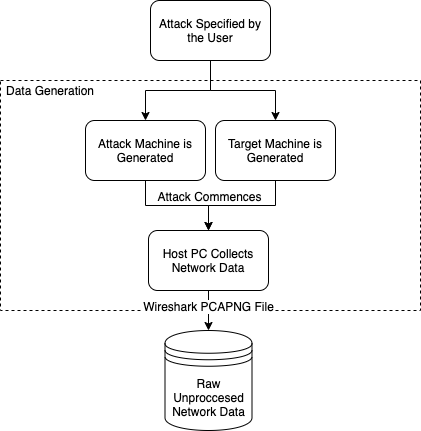
\includegraphics[scale = 0.5]{Images/datagen.png}
 \caption{Data Generation Diagram}
 \label{fig:dgd}
\end{figure}

\subsection{Virtual Machines}
\subsubsection{Virtual Machines Specification}

As seen in the systems diagram in Figure \ref{fig:osd} and in Figure \ref{fig:dgd} the project requires the generation of two virtual machines, namely the attack virtual machine and the target virtual machine. These two virtual machines become the virtualised network that will run the attack scenario.

The attack machine will run Kali Linux, a version of Linux that is tailored towards penetration testing and used widely in the cybersecurity community. This will mean a larger range of tools available for generating attack data and will allow future expandability of the project to contain a larger range of attacks. 

The target machine will run Windows 7, which makes up over 31\% of the operating system market share as of the time of writing \cite{osms}. Windows 7 is also commonly used within offices and is no longer supported by Microsoft as of January 14, 2020. The lack of support and the relatively high usage means that there are many unsecured PCs that could be attacked.

\begin{figure}[h]
 \centering
 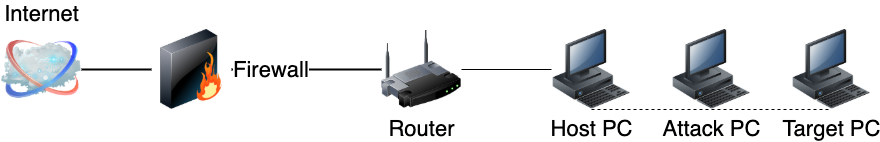
\includegraphics[scale = 0.45]{Images/VM_Network.png}
 \caption{Virtualised Network Diagram }
 \label{fig:vnd}
\end{figure}

The network diagram in Figure \ref{fig:vnd} shows the setup of the virtualised network. The host PC is connected to the router in some form, either by a wired connection or by a wireless connection. When the virtual machines are initialised they will connect to the router via a bridged connection. A bridged connection allows the virtual machines to be on the same network as the host PC and allows the host PC to communicate to the virtual machines.

\subsection{Packer}
Once the virtual machines have been created, as per the above specification, the next part requires the automatic generation of these machines. An open source tool called Packer will facilitate this. Packer was created to automate the creation of virtual machine images.\cite{pckr}. The user supplies two things, namely a template and a packer script.

A template for a virtual machine may be a pre-configured virtual machine, a separate image of this virtual machine or an ISO file, a file which containing an image of a CD containing the operating system to be installed to the virtual machine. 

A packer script is a configuration file which contain certain parameters which allow Packer to locate the virtual machine image, configure the image and build the machine. The configuration file contains three main sections, namely builders, communicators and provisioners \cite{pckr_doc}.

Packer uses a builder to build the virtual machine from some image. Packer can build virtual machines from VirtualBox\cite{pckr_doc}. This can be done directly from a virtual machine, from an Open Virtualisation Format (OVF) file or from an ISO file. This project will use the OVF file to create the machine because it allows greater possible portability of the project without the time sink of setting up virtual machines from scratch.

A communicator allows the host PC to communicate with the virtual machine to execute some commands. This can be done either via Secure Shell (SSH) or via Windows Remote Management (WinRM).\cite{pckr_doc} The host PC must be on the same network as the virtual machine for this to work as there must be a communication path between the virtual machines and the host PC.

Once a connection has been made, a provisioner is used to execute some actions in the virtual machine automatically. There are many provisioners available such as Shell, Ansible, Puppet and Chef among others.\cite{pckr_doc}. The project will use attacks which are written in shell scripts therefore requiring the use of the shell provisioner. Listing \ref{code:pckr_shell} form the packer documentation shows how the shell provisioner is used. A shell script, contained in the host PC, is specified and can run within the virtual machine.
\begin{lstlisting}[language = json, caption = Packer Shell Example, label=code:pckr_shell]
{
     "type": "shell",
     "script": "script.sh",
     "pause_before": "10s",
     "timeout": "10s"
}
\end{lstlisting}
Once a valid packer script has been written and a valid template exists, then packer can build the virtual machine by running the command:
\begin{verbatim}
 packer build template.json
\end{verbatim}
\subsection{Attacks}
Once the virtual machines are generated then attack scripts can be utilised to generate the required network data to build the dataset. 
\begin{table}[H]
 \caption{List of attacks}
 \label{table:attacks}
 \begin{tabular}{|c|c|l|}
 \hline
 \textbf{Attack}&\textbf{Tool}&\textbf{Command} \\
 \hline
 Normal& web-generator & \texttt{pyhton3 gen.py}\\
 \hline
 Syn Flood& Metasploit& \texttt{msfconsole -q -x "use auxiliary/dos/}\\
 &&\texttt{tcp/synflood;set RHOST IP;exploit;"}\\
 \hline
 FIN Flood&Hping&\texttt{hping3 --flood --rand-source -F -p }\\
 &&\texttt{PORT IP}\\
 \hline
 UDP Flood&Hping&\texttt{hping3 --flood --rand-source --udp -p }\\
 &&\texttt{PORT IP}\\
 \hline
 PSH \& ACK Flood&Hping&\texttt{hping3 --flood --rand-source -PA -p}\\
 &&\texttt{PORT IP}\\
 \hline
\end{tabular}
\end{table}
The attacks seen in Table \ref{table:attacks} will be used in the project. They were generated a few different techniques which were all present on the Kali Linux Distribution.

\subsubsection{Normal}
For any anomaly detection system to function correctly, the model must understand normal behaviour. Normal network usage can comprise many things. To best simulate normal network data, an open source python script called web-traffic-generator is used\cite{wtg}. A user on GitHub created this script, which sends HTTP requests to links that are found on the root-url in a pre-defined list of URLs. The script therefore aims to simulate a user browsing the Internet to allow the generation of organic, normal network data.

\subsubsection{SYN Flooding}
The first DoS attack that will be used is a synflood attack. The attack forms a general TCP connection with a TCP handshake. There are three key steps to the TCP handshake\cite{tcp_hand}:

\begin{enumerate}
\item The client sends a Synchronisation Sequence Number (SYN) informing the server the sequence number the connection will be made with

\item The server sends a response with the SYN-ACK flags set.

\item The client responds with the ACK flag set which enables a connection to happen
\end{enumerate}

The syn attack works by sending a large amount of SYN packets to the server. The server then has to keep the connection alive for each packet of these requests. This ensures that the server resources are all taken up with these requests\cite{syn}. An example can be seen in Figure \ref{fig:esfpr}.

\begin{figure}[H]
    \centering
    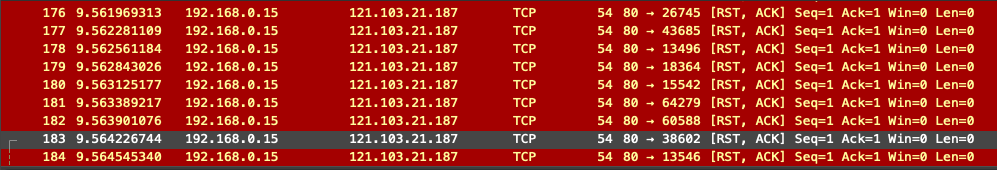
\includegraphics[scale = 0.4]{Images/synflood.png}
    \caption{Example synflood packets}
    \label{fig:esfpr}
\end{figure}

The tool used is Metasploit which is a penetration testing tool with an extensive list of exploits which can be used in a multitude of attacks.\cite{metasploit} 

\subsubsection{FIN Flood}
A FIN flooding attack is a DoS attack which floods the user with TCP packets which have the FIN flags set. The FIN flag indicates that the client is finished and there are no more packets to send. When a FIN packet is received the server and client have started a four-way termination handshake. This handshake starts with a FIN packet from the client, the server responds with an ACK packet and a FIN packet, which the client acknowledges. As the connection does not actually exist the FIN flood will cause the server to try to reset the connection and acknowledge the previous packet which ensures that the servers resources are again taken up. 

The tool used is Hping, which is another network security tool used mainly for penetration testing networks.\cite{hping}

\subsubsection{PSH \& ACK Flood}
When a server receives a packet with the ACK flag set, the server must respond with a confirmation that the packet was received successfully. When a server receives a packet with the PSH flag set, the server must process the information within the packet. Both flags means that the server has to do a lot of processing. When the processing is done the server will reset the connection to respond to the extra requests, all of this will take up large amounts of the server’s resources.

\subsubsection{UDP Flood}
A UDP flood follows a similar path to previous flood attacks. The attack aims to take advantage of how servers respond to UDP packets.\cite{udp} The server checks if any programs are listening on that port, if there are none, it sends an ICMP packet to inform the client that the port is closed. The server is therefore preoccupied with sending ICMP packets in response to the attack that most of the resources will not be available to legitimate users of the server.

\subsection{Data Collection}
After the network data can be generated there must be a way to collect the network data. For this the open source software known as Wireshark. Wireshark is a packet analyser which allows for the collection of packets which are being sent and are received on the network. Wireshark functions by putting the network interface into promiscuous mode, which allows it to see all of the incoming and outgoing network traffic.
 
\section{Data Processing}\label{sec:datapro}
This part of the project is directed around the parsing of the data amassed from section \ref{sec:datagen}, selecting useful features from the data and building a dataset. The raw network data which was generated in section \ref{sec:datagen} will be processed by, first filtering the packets to only contain those which arrived to or came from the virtual machines. Features are then extracted from these packets and are then collated so that the features are counted every second.

\begin{figure}[H]
 \centering
 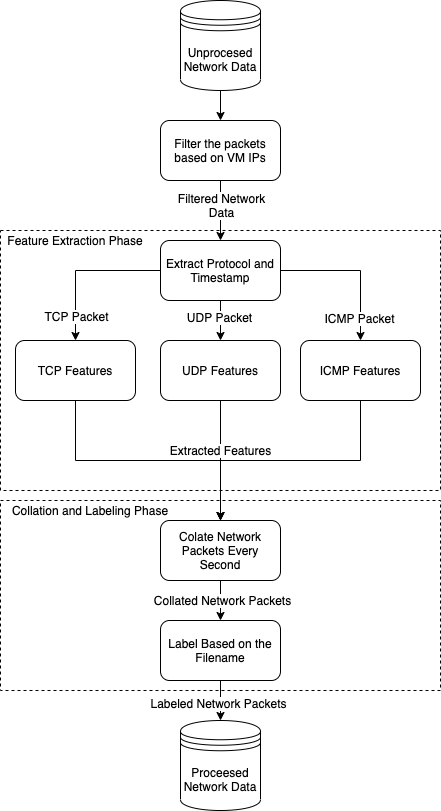
\includegraphics[scale = 0.5]{Images/datacollection.png}
 \caption{Data Collection Diagram}
 \label{fig:dcd}
\end{figure}
\subsection{Feature Extraction Phase}

Once the network data has been generated and collected with wireshark, it creates a PCAP Next Generation Dump (PCAPNG) File. This file type is the native file type for wireshark and contains all the network data generated from an attack. Wireshark collects the network data of the Host PCs network. As this network will contain noise from other machines connected to it, the data must first be filtered. Since an intrusion detection system will mainly run on the target PC, the filtering will only include packets that are sent to and received from the target machine. Wireshark allows filtering network data using DisplayFilters \cite{filters}. 

\begin{verbatim}
 ip.addr == 192.168.0.15
\end{verbatim}

The filter above will only keep packets that came to or arrived from the target machine. This can be achieved by setting a static IP for the target machine image so that the IP address will never change. This means that all the packets in the collection will be from the attack and will thus will limit noise. While it can do this in wireshark, it does not automate it. For the automation of the process, a library needs to be used to extract the packets and store the important pieces of data into a CSV file. 

\subsubsection{Pyshark}
Pyshark is an open source python library which wraps tshark\cite{pyshark}, tshark is a terminal-based version of wireshark which can allow for parsing out network data from PCAPNG files. This project uses pyshark version 0.4.2.9 which was released on Aug 11, 2019.

\begin{lstlisting}[language = python, caption = Pyshark Example Code, label=code:pyshrk]
import pyshark
self.cap = pyshark.FileCapture(input_file="normal.pcapng", 
 display_filter =filter)
# Write the packets
for packet in self.cap:
\end{lstlisting}

The Code seen in Listing \ref{code:pyshrk} shows an example of reading a network file. Once these packets are read then they can be looped through one by one and the features extracted. From here they can all be stored as a CSV file or stored in an array to be manipulated later.

\subsection{Feature Selection}

One of the most essential parts of building a machine learning algorithm is feature selection. Feature selection refers to the act of choosing features in your dataset that best contribute to the target class. Performing good feature selection will allow a much cleaner model, which is less prone to overfitting and improves accuracy.\cite{feat_select}.

\begin{table}[H]
 \centering
 \caption{List of Features to be Extracted Initially}
 \label{table:features_init}
 \begin{tabular}{|c|c|}
 \hline
 \textbf{Feature}&\textbf{Data Type}\\
 \hline
 Timestamp & Date \& Time \\
 \hline
 Protocol & Integer\\ 
 \hline
 Source Port & Integer\\
 \hline
 Destination Port & Integer\\
 \hline
 TCP Finish Flag & Binary Value\\
 \hline
 TCP Synchronise Flag & Binary Value\\
 \hline
 TCP Push Flag & Binary Value\\
 \hline
 TCP Acknowledge Flag & Binary Value\\
 \hline
 TCP Urgent Flag & Binary Value\\
 \hline
\end{tabular}
\end{table}

The features seen in Table \ref{table:features_init} are the features which are initially extracted from the network data. For a DoS attack, it is important to know what type of protocol was used and what flags were set, from this the DoS attack can be determined. However, on their own these features are not enough as a single packet gives no context about what is happening within the network, to better distinguish what is going on within the network the packets must be collated within a time frame to lend some context to the packet.

In their paper, P.Sangkatsanne et al. \cite{SANGKATSANEE20112227} found 12 features that best differentiated the attacks they used. They did this using information gain, as seen in the literature review.

\begin{table}[h]
 \centering
 \caption{List of Features from P.Sangkatsanne et al.}
 \label{table:features}
 \begin{tabular}{|c|c|}
 \hline
 \textbf{Feature}&\textbf{Data Type}\\
 \hline
 Number of TCP packets & Integer \\
 \hline
 Number of TCP source ports & Integer\\ 
 \hline
 Number of TCP destination port & Integer\\
 \hline
 Number of TCP finish flag & Integer\\
 \hline
 Number of TCP synchronise flag & Integer\\
 \hline
 Number of TCP push flag & Integer\\
 \hline
 Number of TCP acknowledge flag & Integer\\
 \hline
 Number of TCP urgent flag & Integer\\
 \hline
 Number of UDP packets & Integer\\
 \hline
 Number of UDP source port & Integer\\
 \hline
 Number of UDP destination port & Integer\\
 \hline
 Number of ICMP packets & Integer\\
 \hline
\end{tabular}
\end{table}

The features seen in Figure \ref{table:features} are the features which are extracted from the network data, these features are aggregated every 2 seconds. The paper claims that these features will be able to sufficiently classify DoS and Probe attacks. As this paper will mainly focus on DoS attacks, these features should differentiate between them.

The timestamp seen in Table \ref{table:features_init} will be used to collate the network packet features into one second data points. 
\subsection{Collation and Labeling Phase}
Once the features of each individual packet are extracted they must be collated, and the features seen in Table \ref{table:features} extracted from them.
\subsubsection{Pandas}
The Python Data Analysis Library (Pandas) is a python library that deals with data manipulation and analysis. Pandas will take some data from a data type such as a CSV or a list and create a Dataframe. A dataframe is a 2D labelled data structure that resembles a spreadsheet \cite{pandas_docs}. Dataframes allow easier indexing by time and can quickly apply functions to an entire column instead of looping through each data point in the dataset.

Here pandas can collate the network data into dataframes which contain the packets in a particular second. From here, it can apply operations to extract the features from the packets, as in Table \ref{table:features}. These can then be written to a CSV containing the previous attack data to generate a dataset.
\subsubsection{Labeling}
Each network file is stored with the name of the attack, this filename can be used to label the attacks once the network packets are processed.
\section{Data Modeling}
This part of the project is focused on using the processed data from section \ref{sec:datapro} to train a machine learning model. The processed network data will be split into training and test data to ensure no overfitting, and a model is trained from this data. From the literature review, the consensus is that a decision tree model would perform best for Intrusion detection.
\subsection{Scikit Learn}
Python has many packages to use for machine learning but the one which supports the most algorithms is scikit learn. scikit learn is a python library which implements multiple machine learning algorithm including a decision tree algorithm by implementing the CART algorithm. scikit learn is very simple to use and is compatible with pandas so the network data can be read and can train the classifier. This project uses scikit learn version 0.22.2 released on Mar 4, 2020.
\begin{lstlisting}[language = python, caption = Decision Tree scikit-learn Example, label=code:skit]
from sklearn import tree
X = [[0, 0], [1, 1]]
Y = [0, 1]
clf = tree.DecisionTreeClassifier()
clf = clf.fit(X, Y)
\end{lstlisting}
The code seen in Listing \ref{code:skit} is an example implementation of a decision tree classifier taken from the documentation \cite{scikit}. The code is easy to implement and creates a good classifier that can be used in production.\cite{scikit_prod}. 

